%!TEX root = ../report.tex

\begin{document}
    \chapter{Solution}

   \section{Hand crafted feature extraction}  
   First approach to analyze and explore the domain knowledge of the raw signal from accelerometer is calculating temporal, spectral and statistical aspects of the data. As discussed in chapter 3 domain specific knowledge can be extracted from time-series data to analyze it and used as input to machine learning algorithms as raw signal cannot be used directly. Along with the calculated features we have prior information that has been extracted from the signal that is, penetration and maximum velocity. The dataset contains three signals acceleration, velocity and position that are passed to feature extractor which extracts fixed set of features.
   
      \begin{figure}
      	\centering
      	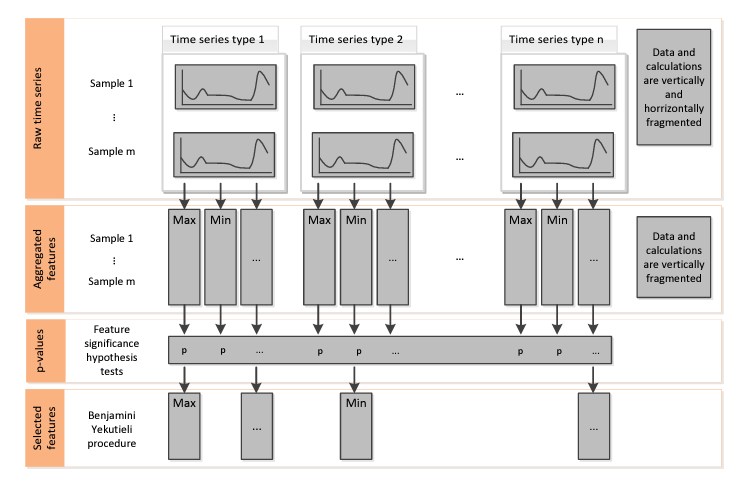
\includegraphics[width=1.2\linewidth]{images/hcta.png}
      	\caption{Process of extracting features from time-series data \cite{christ2016distributed}}
      	\label{n0}
      \end{figure}
   
   \begin{table}[h]
   	\centering
   	\begin{tabular}{|l|l|}
   		\hline
   		Type    & Features                                                                                                                                                                      \\ \hline
   		Statistical & \begin{tabular}[c]{@{}l@{}}Minimum, Maximum, Median, Mean absolute deviation, \\ Median absolute deviation, \\ Root mean square, Standard deviation, \\ Variance\end{tabular} \\ \hline
   		Temporal    & \begin{tabular}[c]{@{}l@{}}Mean absolute differences, Mean differences, \\ Median differences, Median absolute differences,\\  Entropy\end{tabular}                           \\ \hline
   		Spectral    & \begin{tabular}[c]{@{}l@{}} Minimum frequency, Maximum frequency,  \\Median frequency, Fundamental frequency\end{tabular}                             \\ \hline
   	\end{tabular}
   	\caption{Fixed set of hand crafted features}
   	\label{t1}
   \end{table}
   

   The extractor function returns in total 54 features for each car door instance. Table \ref{t1} gives the overview of features calculated for each signal. The dimensionality of the feature vector obtained for each signal is reduced by removing the redundant features and selecting relevant ones by use of Random forest algorithm. This information is passed to supervised machine learning algorithm for classification.
   
   \section{Autoencoder for anomaly detection}   
   To apply a general classification approach there is a requirement of fixed number of classes to separate the data. The problem that is solved by this project contains two classes normal and abnormal. Proper definition of what distinct feature that can classify the signals into these classes is missing. In other words prior information on to what can be called as anomaly is not available because the data we are dealing with is a complex industrial dataset.  Also the data that is provided is highly imbalanced which has been seen during the data analysis in section $4.2.1$. Therefore a direct implementation of deep-learning algorithm to this problem is difficult. These problems arise when we try to find a classification algorithm to solve the problem. To overcome these issues we propose to re frame the problem as anomaly detection using autoencoder.
   
    \begin{figure}[h]
    	\centering
    	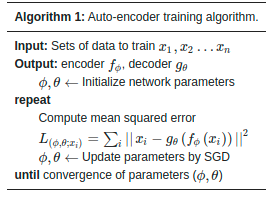
\includegraphics[width=0.5\linewidth]{images/algau.png}
    	\caption{Algorithm for anomaly detection \cite{oh2018residual} }
    	\label{nv0}
    \end{figure}
    
     \begin{figure}[h]
     	\centering
     	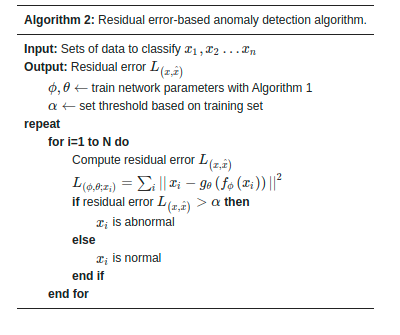
\includegraphics[width=0.75\linewidth]{images/rsd.png}
     	\caption{Algorithm for anomaly detection \cite{oh2018residual} }
     	\label{n00}
     \end{figure}
   
   Detailed discussion on general structure of autoencoder is done in chapter 3 section $3.1.3$. The model is based on low-dimensional latent space which has high level abstraction of features. We do not require prior knowledge of latent variables in order to identify anomalies or outliers. Therefore as prior knowledge is not available for comfort door dataset general autoencoder is suitable for this problem.
   
   The network has same number of inputs and outputs. The goal of this network is to minimize the reconstruction error between the decoded signal and the original. The problem now can be re-framed as regression rather than classification thus mean squared error is suitable for the problem to be solved.     
   
    
    During compression and expansion, the auto-encoder minimizes the loss of information. Although the decoder restores the high-frequency components to their maximum, the loss of the high-frequency components occurs during the compression process of the encoder. Signals are sampled for each element and reconstructed with the goal of reducing the average difference between input and output signals. The reconstructed signal is not equivalent to the original signal.Instead of focusing on if the input is normal or abnormal the reconstruction error is considered. The algorithm learns higher abstraction of data because of dimension reduction.
    
    In the residual error based anomaly detection algorithm computation of the threshold is done based on the validation set. A optimal threshold can be selected if the it is computed based on abnormal data. A trained auto-encoder will predict the unseen normal data with small reconstruction error as the distribution of samples is similar. When it predict anomalous data the reconstruction error is high. Thus reconstruction error acts a aid to catch the rare events. 
    Figure \ref{ne11} shows the architecture of autoencoder model used. 
   
   \begin{figure}[h]
   	\centering
   	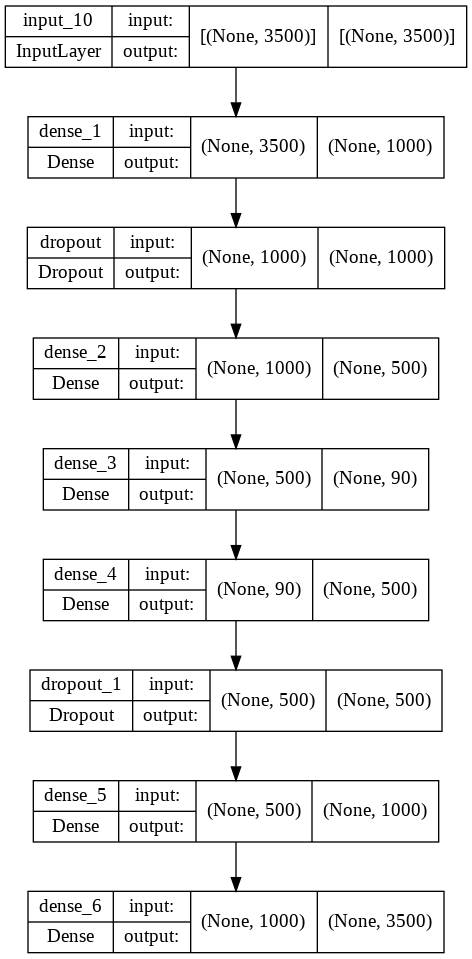
\includegraphics[width=0.49\linewidth]{images/aaut.png}
   	\caption{Autoencoder architecture for anomaly detection }
   	\label{ne11}
   \end{figure}
  
   \section{Transfer learning with raw signal data}
There are very few open source resources trained model which has similar data structure to the complex industrial dataset used for this project. As discussed in the state of art the most popularly used transfer learning model for time series data is CNNs. Many variations of the this model can be found. The model which is used deep convolution network trained with data shown in figure \ref{ne1}. This architecture is chosen based from the paper \cite{fawaz2018transfer}

  \begin{figure}[h]
  	\centering
  	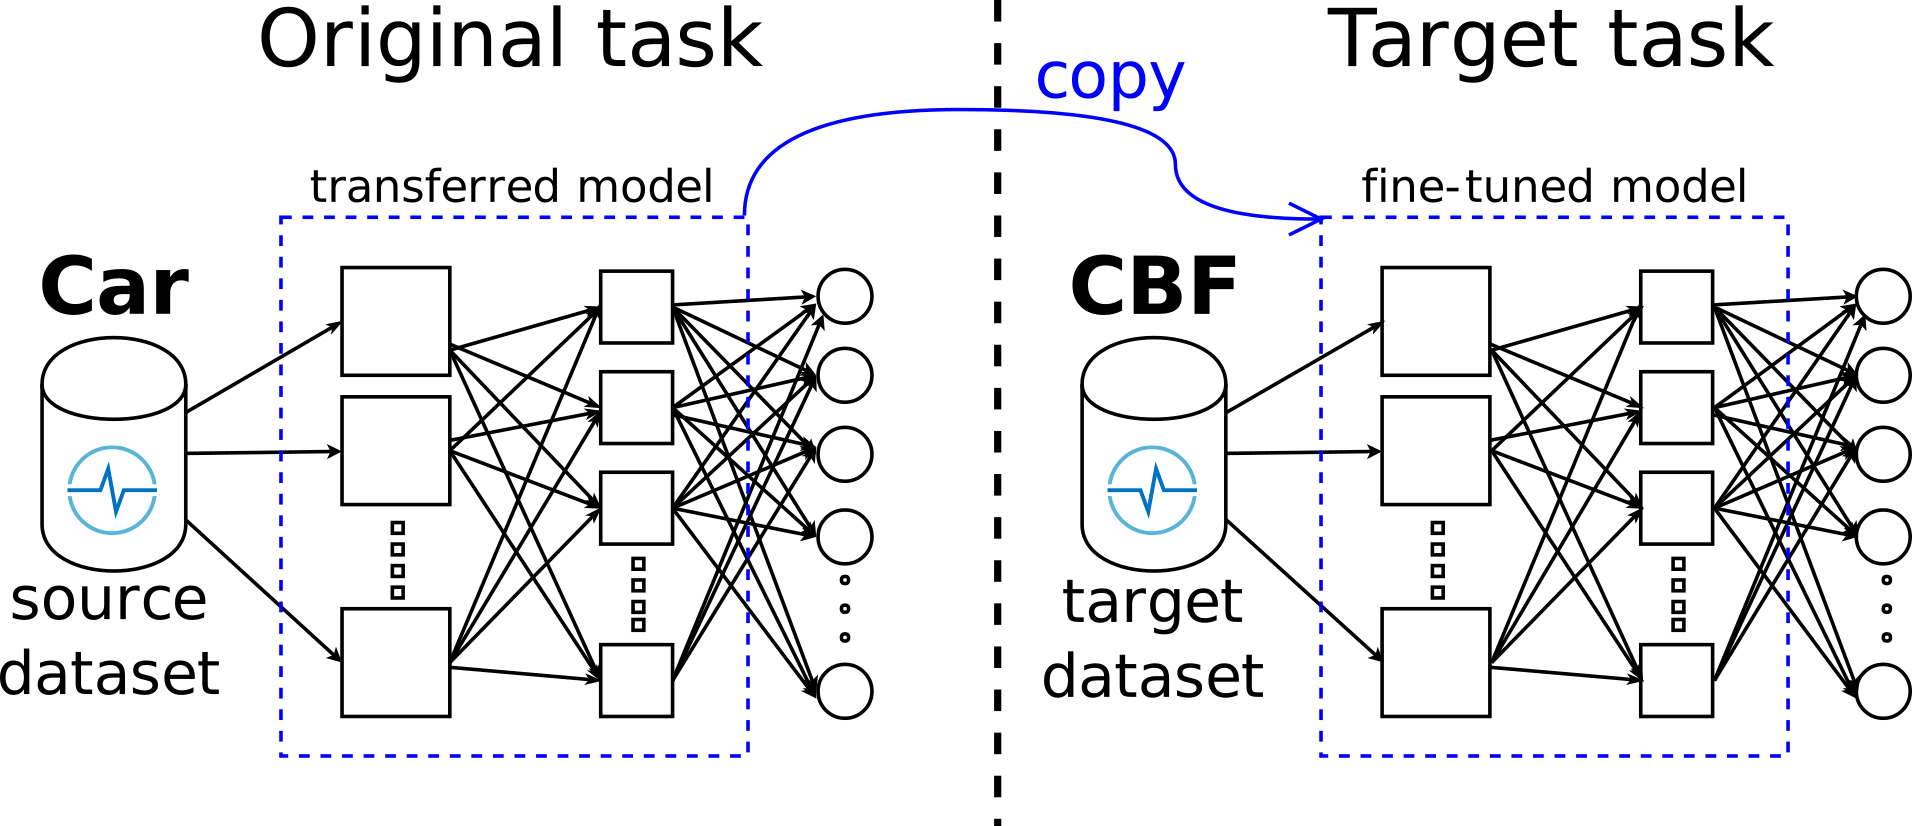
\includegraphics[width=0.9\linewidth]{images/transferss.png}
  	\caption{Transfer learning model \cite{oh2018residual} }
  	\label{n01}
  \end{figure}
   
   \begin{figure}[h]
     	\centering
     	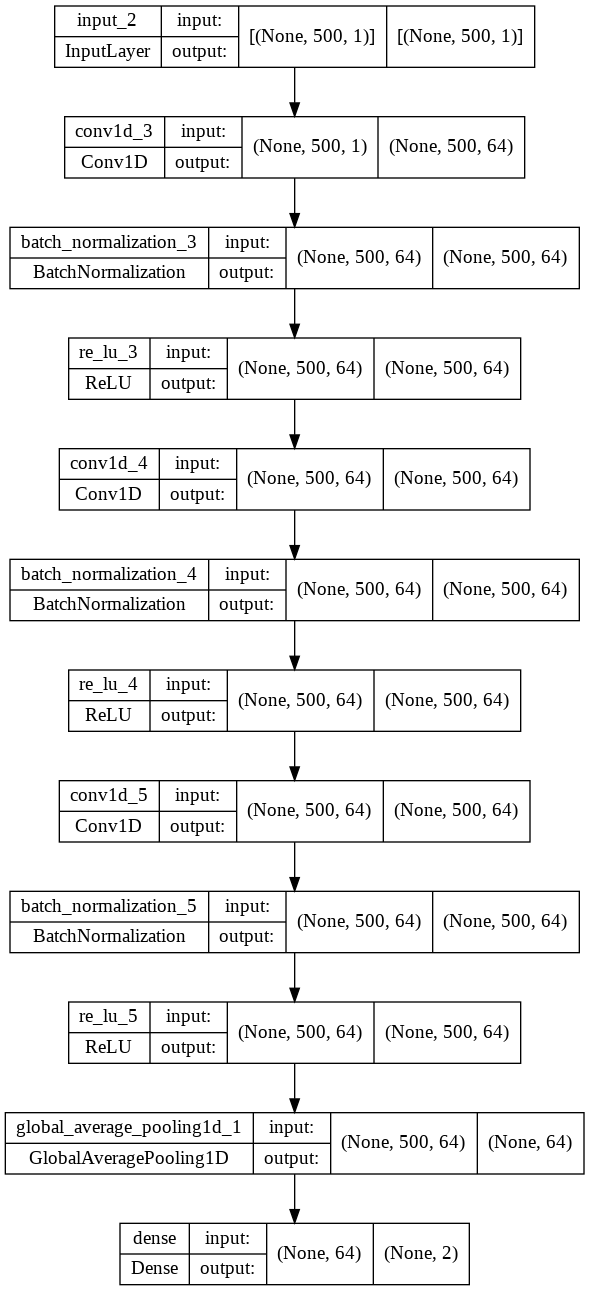
\includegraphics[width=0.49\linewidth]{images/cnna.png}
     	\caption{CNN architecture for transfer learning }
     	\label{ne1}
     \end{figure}
     
   The steps that are followed for use of transfer learning using the above model from raw time series data are as follows:
   \begin{enumerate} 
   	\item As it can be seen in the figure \ref{n01} the model is copied along with its weights.
   	\item The acceleration signal from time series data is resized according to the model input requirements. 
   	\item First few layers of the model are frozen.
   	\item The frozen part acts as feature extractor and this is classified by the model parameters that  are trainable.
   	\item Instead of softmax sigmoid function has been used due to presence of only two classes for the problem.
     \end{enumerate}  
   
 
   \section{Transfer learning with spectrogram}   
  There is a significant work done to designing networks to classify and extracting features from spectrogram. Finding a suitable deep-learning model when we have low instances of data is difficult. Therefore transfer learning is helpful solving this problem. Various popular networks architectures such as VGG and Resnet have been used to extract features from spectogram data. For this project VGG is used. 
  
  VGG which is a image classification model and has no relation to the temporal domain knowledge in its design. Also as discussed earlier a clear definition to anomaly is missing. Even with these issues VGG is suitable for this problem because, not considering the domain knowledge minimizes the assumptions that are done with respect to the specific domain. Deep learning models are known to be perming better if the feature space is not constrained with domain knowledge. Rather than make assumptions about the type of signal or problem, VGGs combine small-context representations all hierarchically, so that any structure can be learned \cite{vgg}. 
  
  The steps that are followed for use of transfer learning from spectrogram are as follows:
  \begin{enumerate}
  	\item First step is to pre-process the image in such a manner that it is in suitable format of input for VGG network. Required input shape for the network is $(244,244,3)$. Also the data should be normalized to values $0$ to $1$ by dividing the array with factor of $225$.

  	\item Next step is to load VGG model with pre-trained weights for imgenet dataset.  
  	
  	\item  The feature extractor part of the network is defined from the network input to the last max pooling layer (labeled by 7 x 7 x 512). The remaining part is regarded as the classification part.The feature extraction part of the model is frozen to ensure the weights of the network do not change during model training.
  	
  	\item To scale and convert the image into Numpy array module from Keras \cite{ketkar2017introduction} library has been used.
  	
  	\item The classification part of the network is trained with the features obtained from the extractor part of the network.
  	
    \item Instead of softmax sigmoid function has been used due to presence of only two classes for the problem.
  \end{enumerate}
  
  
  \section{Autoencoder as feature extractor}  
     \begin{figure}[h]
     	\centering
     	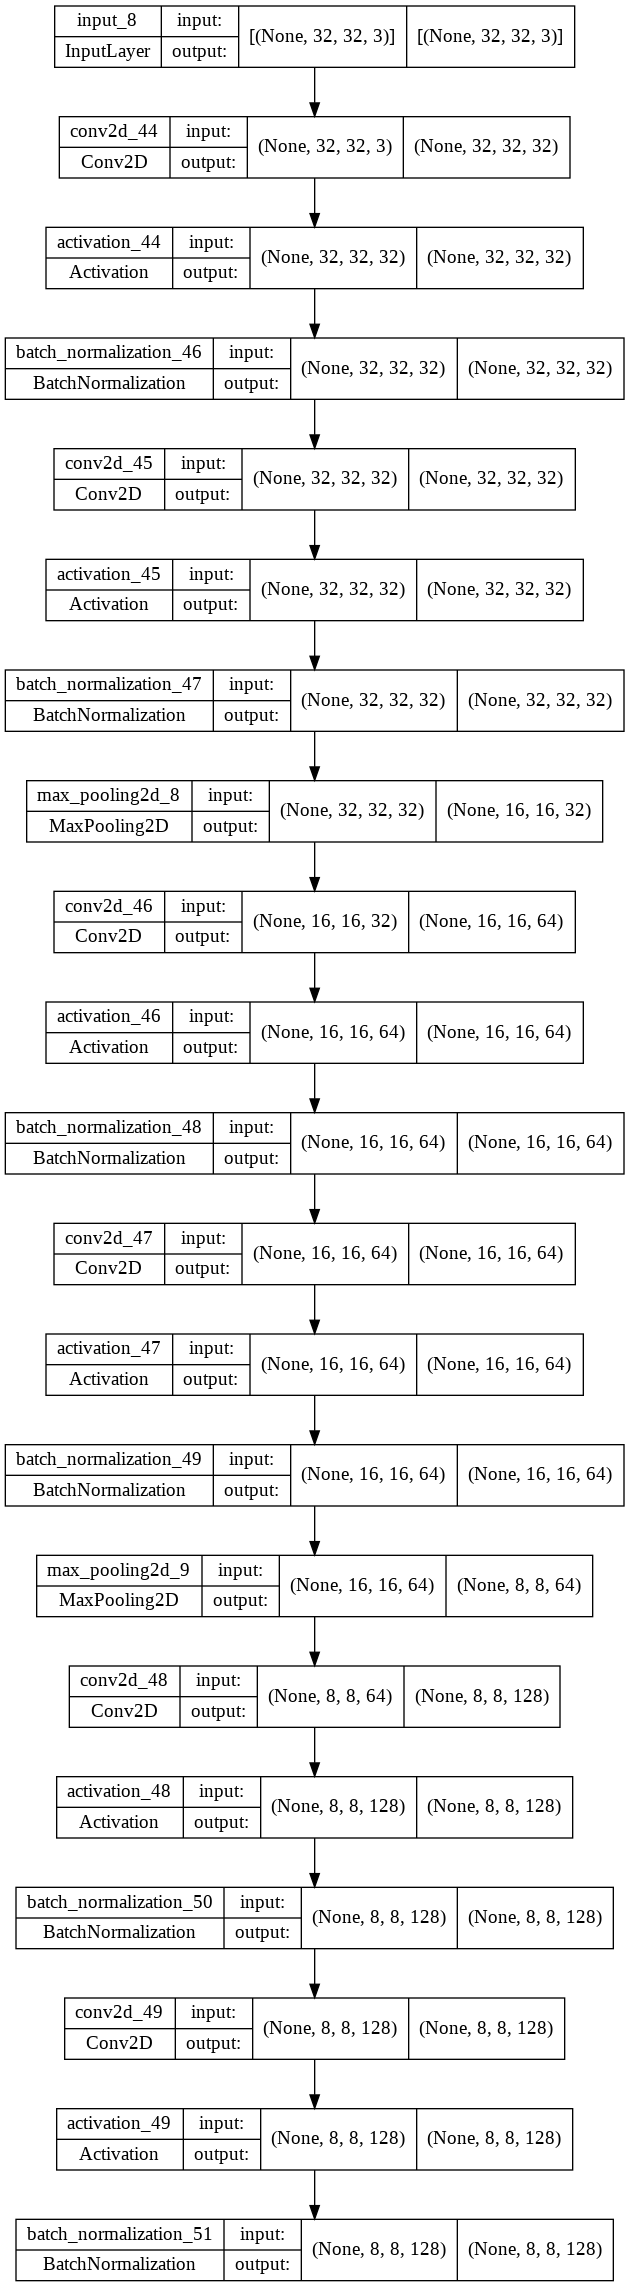
\includegraphics[width=0.35\linewidth]{images/encoder.png}
     	\caption{Encoder architecture }
     	\label{ne1}
     \end{figure}
     
   

\end{document}
